\documentclass[tikz]{standalone}

\usepackage{tikz}
\usetikzlibrary{arrows.meta}
\usetikzlibrary{decorations.pathreplacing}

% Female/male symbols
\usepackage{wasysym}

% For tables
\usepackage{booktabs}

% For dashed lines
\usepackage{arydshln}

\begin{document}

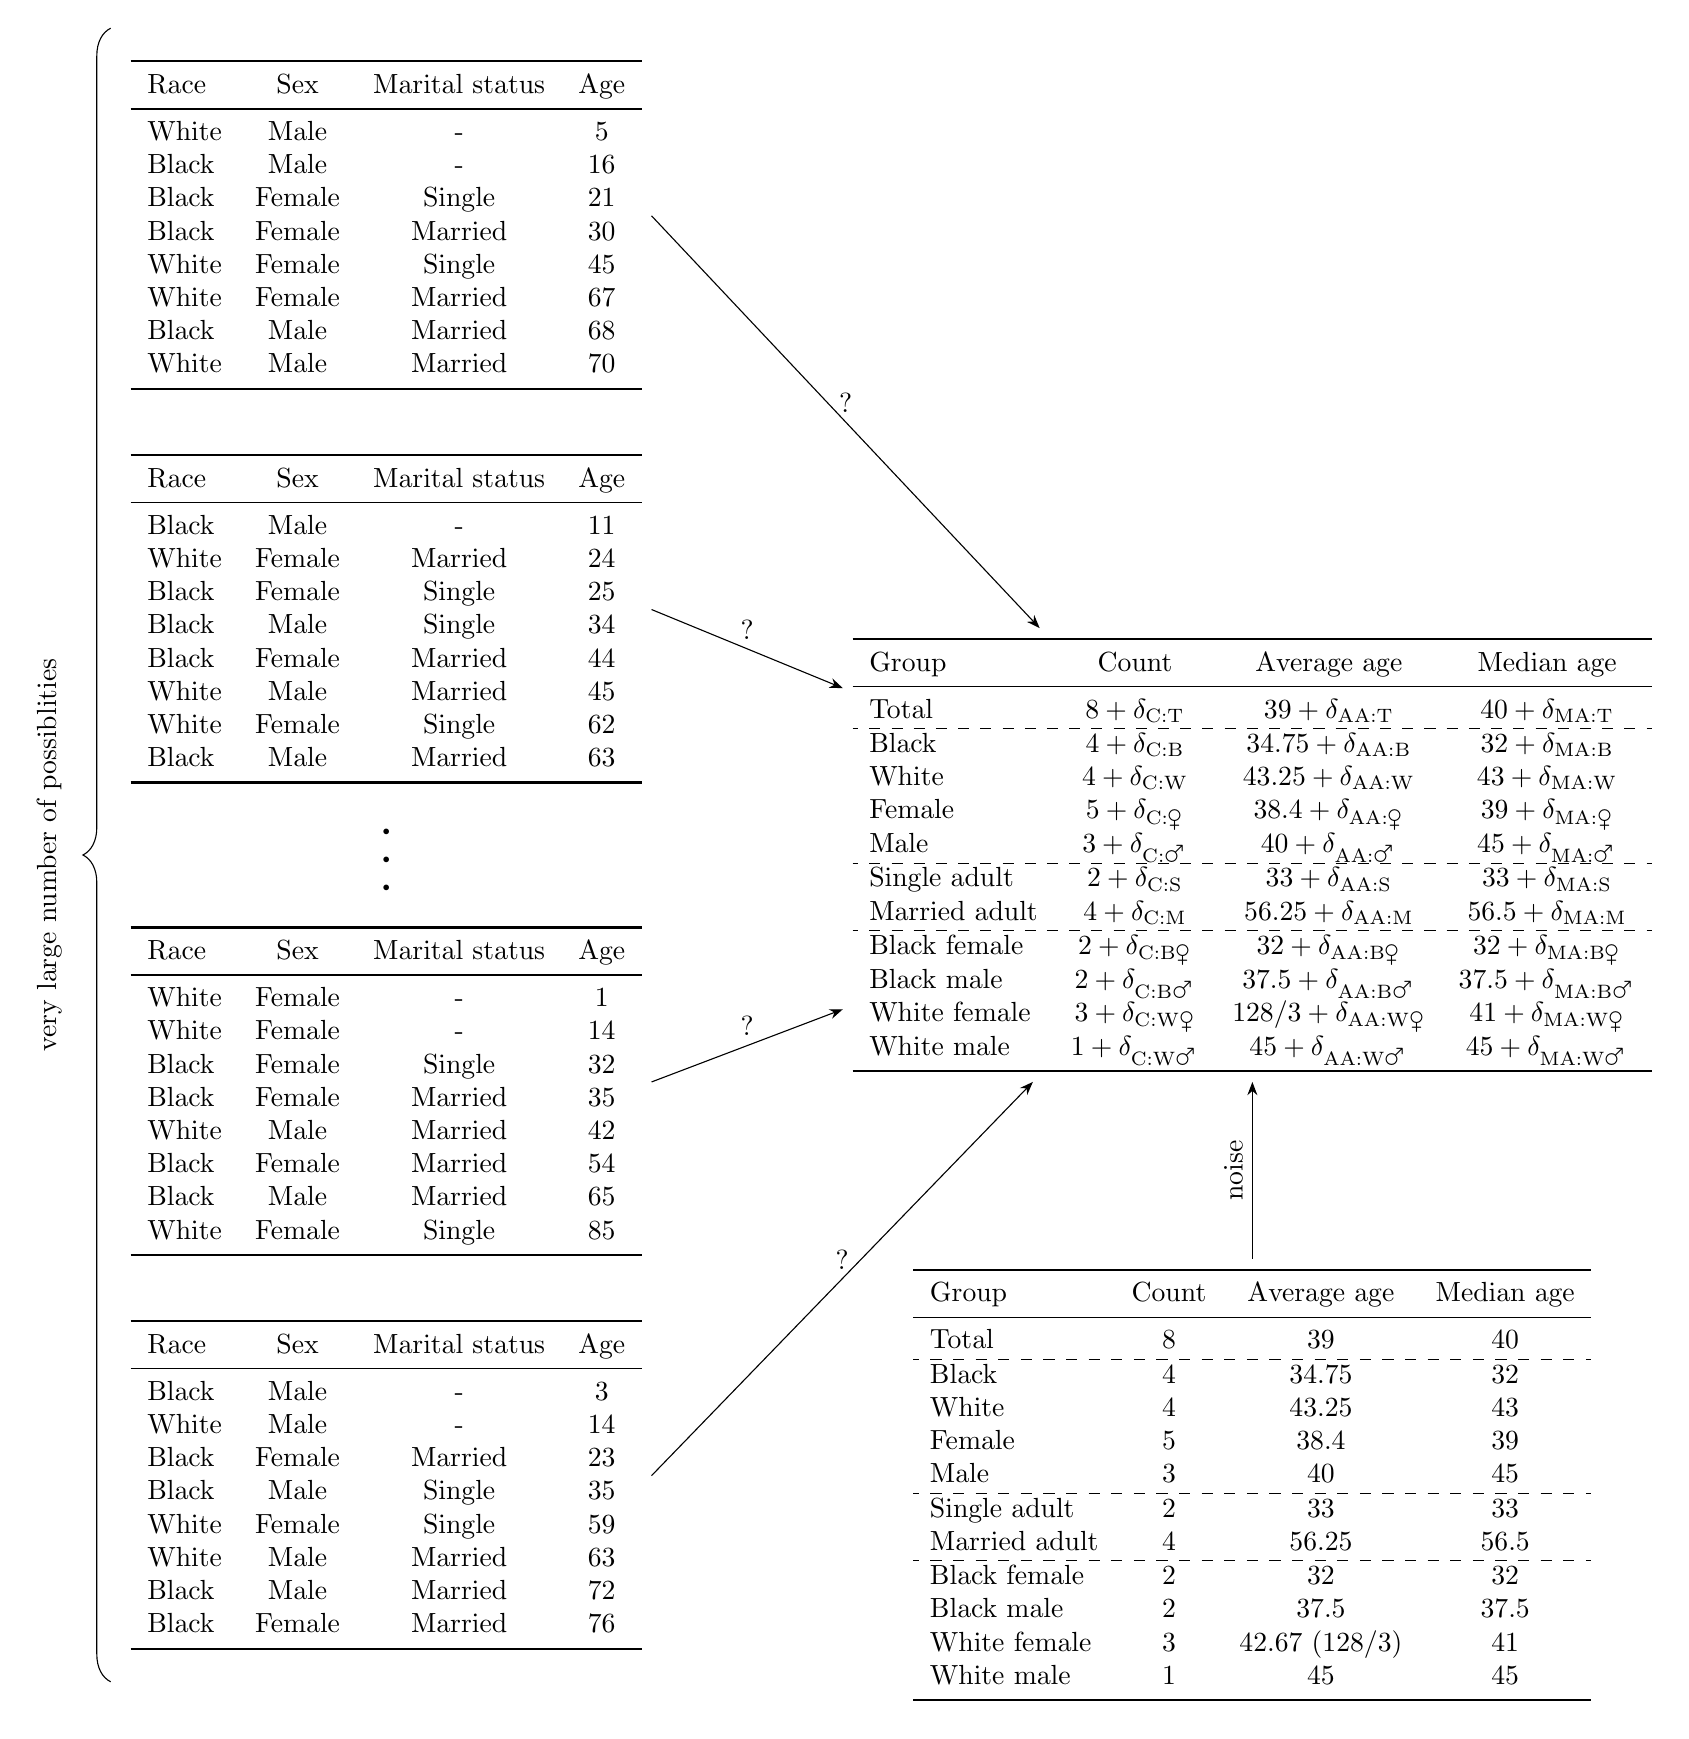
\begin{tikzpicture}[>=Stealth]
  \node (individuals-table-1) at (0, 8) {%
      \begin{tabular}{lccc}
	\toprule
	Race  & Sex    & Marital status & Age \\
	\midrule
	White & Male   & -              & 5   \\
	Black & Male   & -              & 16  \\
	Black & Female & Single         & 21  \\
	Black & Female & Married        & 30  \\
	White & Female & Single         & 45  \\
	White & Female & Married        & 67  \\
	Black & Male   & Married        & 68  \\
	White & Male   & Married        & 70  \\
	\bottomrule
      \end{tabular}
    };

  \node (individuals-table-2) at (0, 3) {%
      \begin{tabular}{lccc}
	\toprule
	Race  & Sex    & Marital status & Age \\
	\midrule
	Black & Male   & -              & 11  \\
	White & Female & Married        & 24  \\
	Black & Female & Single         & 25  \\
	Black & Male   & Single         & 34  \\
	Black & Female & Married        & 44  \\
	White & Male   & Married        & 45  \\
	White & Female & Single         & 62  \\
	Black & Male   & Married        & 63  \\
	\bottomrule
      \end{tabular}
    };

  \node (individuals-table-n-1) at (0, -3) {%
      \begin{tabular}{lccc}
	\toprule
	Race  & Sex    & Marital status & Age \\
	\midrule
	White & Female & -              & 1   \\
	White & Female & -              & 14  \\
	Black & Female & Single         & 32  \\
	Black & Female & Married        & 35  \\
	White & Male   & Married        & 42  \\
	Black & Female & Married        & 54  \\
	Black & Male   & Married        & 65  \\
	White & Female & Single         & 85  \\
	\bottomrule
      \end{tabular}
    };

  \node (individuals-table-n) at (0, -8) {%
      \begin{tabular}{lccc}
	\toprule
	Race  & Sex    & Marital status & Age \\
	\midrule
	Black & Male   & -              & 3   \\
	White & Male   & -              & 14  \\
	Black & Female & Married        & 23  \\
	Black & Male   & Single         & 35  \\
	White & Female & Single         & 59  \\
	White & Male   & Married        & 63  \\
	Black & Male   & Married        & 72  \\
	Black & Female & Married        & 76  \\
	\bottomrule
      \end{tabular}
    };

  \node (summary-table) at (11, -8) {%
      \begin{tabular}{lccc}
	\toprule
	Group & Count & Average age & Median age \\
	\midrule
	Total         & 8 & 39              & 40   \\
	\hdashline
	Black         & 4 & 34.75           & 32   \\
	White         & 4 & 43.25           & 43   \\
	Female        & 5 & 38.4            & 39   \\
	Male          & 3 & 40              & 45   \\
	\hdashline
	Single adult  & 2 & 33              & 33   \\
	Married adult & 4 & 56.25           & 56.5 \\
	\hdashline
	Black female  & 2 & 32              & 32   \\
	Black male    & 2 & 37.5            & 37.5 \\
	White female  & 3 & 42.67 ($128/3$) & 41   \\
	White male    & 1 & 45              & 45 \\
	\bottomrule
      \end{tabular}
    };

  \node (summary-table-noisy) at (11, 0) {%
      \begin{tabular}{lccc}
	\toprule
	Group         & Count                     & Average age                    & Median age                  \\
	\midrule
	Total         & $8 + \delta_\mathrm{C:T}$        & $39 + \delta_\mathrm{AA:T}$           & $40 + \delta_\mathrm{MA:T}$        \\
	\hdashline
	Black         & $4 + \delta_\mathrm{C:B}$        & $34.75 + \delta_\mathrm{AA:B}$        & $32 + \delta_\mathrm{MA:B}$        \\
	White         & $4 + \delta_\mathrm{C:W}$        & $43.25 + \delta_\mathrm{AA:W}$        & $43 + \delta_\mathrm{MA:W}$        \\
	Female        & $5 + \delta_\mathrm{C:\female}$  & $38.4 + \delta_\mathrm{AA:\female}$   & $39 + \delta_\mathrm{MA:\female}$  \\
	Male          & $3 + \delta_\mathrm{C:\male}$    & $40 + \delta_\mathrm{AA:\male}$       & $45 + \delta_\mathrm{MA:\male}$    \\
	\hdashline
	Single adult  & $2 + \delta_\mathrm{C:S}$        & $33 + \delta_\mathrm{AA:S}$           & $33 + \delta_\mathrm{MA:S}$        \\
	Married adult & $4 + \delta_\mathrm{C:M}$        & $56.25 + \delta_\mathrm{AA:M}$        & $56.5 + \delta_\mathrm{MA:M}$      \\
	\hdashline
	Black female  & $2 + \delta_\mathrm{C:B\female}$ & $32 + \delta_\mathrm{AA:B\female}$    & $32 + \delta_\mathrm{MA:B\female}$ \\
	Black male    & $2 + \delta_\mathrm{C:B\male}$   & $37.5 + \delta_\mathrm{AA:B\male}$    & $37.5 + \delta_\mathrm{MA:B\male}$ \\
	White female  & $3 + \delta_\mathrm{C:W\female}$ & $128/3 + \delta_\mathrm{AA:W\female}$ & $41 + \delta_\mathrm{MA:W\female}$ \\
	White male    & $1 + \delta_\mathrm{C:W\male}$   & $45 + \delta_\mathrm{AA:W\male}$      & $45 + \delta_\mathrm{MA:W\male}$   \\
	\bottomrule
      \end{tabular}
    };

  \foreach \idx in {1, 2, n-1, n} {%
    \draw[->] (individuals-table-\idx.e) -- node[above] {?} (summary-table-noisy);
  }

  \path (individuals-table-2) -- node[auto=false, rotate=90]{\Huge\ldots} (individuals-table-n-1);

  \draw [decorate,decoration={brace, amplitude=10pt, mirror}, yshift=0pt] (-3.5, 10.5) -- node[rotate=90, above, yshift=0.5cm] {very large number of possiblities} (-3.5, -10.5);
    
  \draw[->] (summary-table) -- node[rotate=90, above] {noise} (summary-table-noisy);

\end{tikzpicture}

\end{document}
